% Friday presentation — mathematics summary (~21 slides)
% Compile: pdflatex presentation_friday.tex (twice)

\documentclass[aspectratio=169,11pt]{beamer}

\usepackage[T1]{fontenc}
\usepackage[utf8]{inputenc}
\usepackage[english]{babel}
\usepackage{lmodern}
\usepackage{amsmath,amssymb}
\usepackage{booktabs}
\usepackage{tikz}
\usetikzlibrary{shapes,arrows.meta,positioning}
\usepackage{url}

\usetheme{AnnArbor}
\usecolortheme{wolverine}
\setbeamertemplate{navigation symbols}{}

\definecolor{triageRed}{RGB}{220, 20, 60}
\definecolor{triageOrange}{RGB}{255, 140, 0}
\definecolor{triageYellow}{RGB}{255, 200, 0}
\definecolor{triageGreen}{RGB}{34, 139, 34}

\newcommand{\bcol}[2][blue!70!black]{\textcolor{#1}{#2}}

\setbeamertemplate{footline}{%
	\hfill\small \insertframenumber{} / \inserttotalframenumber\hspace{1.5em}%
}

\tikzset{
	flowbox/.style={rectangle, draw=black!60, rounded corners=2pt, fill=blue!8,
		minimum height=0.75cm, minimum width=1.6cm, align=center, font=\scriptsize, inner sep=3pt},
	flowarr/.style={-{Stealth[length=2mm]}, thick},
	edgelabel/.style={font=\tiny, fill=white, inner sep=1pt}
}

\title[Friday Presentation]{Hospital Chatbot for Color-Coded Clinical Pathways}
\author{Quaigraine Samuel \and Twum Samuel}
\institute{Department of Mathematics\\Kwame Nkrumah University of Science and Technology}
\date{\today}

\begin{document}

% ========== Part I: Introduction ==========
\begin{frame}
	\titlepage
\end{frame}

\begin{frame}{Contents}
	\tableofcontents
\end{frame}

\section{Introduction and pipeline}

\begin{frame}{From chat and vitals to one triage colour}
	\textbf{Today's question:} How does the system turn what a patient says and what we know about their vitals into \textbf{one} urgency colour?

	\vspace{0.3em}
	\textbf{This talk:} The \textbf{mathematics} behind that decision --- three layers (language, vitals, probability) and a fusion step --- not a repeat of the general project overview.

	\vspace{0.25em}
	\textbf{The colour $C$} follows \textbf{SATS} (South African Triage Scale):
	\begin{itemize}
		\item \bcol[triageRed]{Red} --- immediate, life-threatening
		\item \bcol[triageOrange]{Orange} --- very urgent
		\item \bcol[triageYellow]{Yellow} --- urgent
		\item \bcol[triageGreen]{Green} --- non-urgent
	\end{itemize}

	\vspace{0.25em}
	\footnotesize The system supports triage staff; it does \textbf{not} diagnose disease or replace clinical judgment.
\end{frame}

\begin{frame}{How three mathematical layers produce one triage colour}
	\begin{center}
		\resizebox{0.95\textwidth}{!}{%
		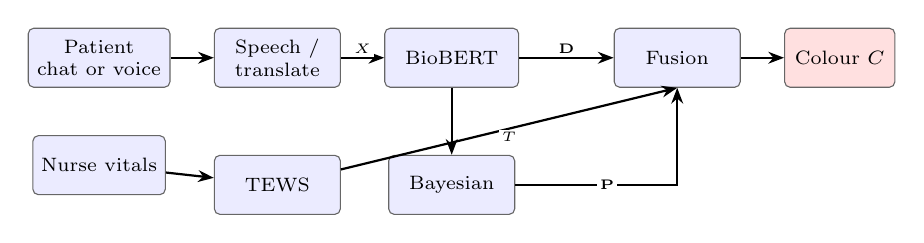
\begin{tikzpicture}[node distance=0.7cm and 0.55cm]
			\node[flowbox, minimum width=1.8cm] (patient) {Patient\\chat or voice};
			\node[flowbox, right=of patient] (lang) {Speech /\\translate};
			\node[flowbox, right=of lang, minimum width=1.7cm] (nlp) {BioBERT};
			\node[flowbox, below=0.85cm of lang] (tews) {TEWS};
			\node[flowbox, below=0.85cm of nlp] (bayes) {Bayesian};
			\node[flowbox, right=1.2cm of nlp, minimum width=1.6cm] (fuse) {Fusion};
			\node[flowbox, right=of fuse, fill=red!12, minimum width=1.4cm] (out) {Colour $C$};
			\node[flowbox, below=0.6cm of patient] (vitals) {Nurse vitals};
			\draw[flowarr] (patient) -- (lang);
			\draw[flowarr] (lang) -- node[edgelabel, above] {$X$} (nlp);
			\draw[flowarr] (nlp) -- node[edgelabel, above] {$\mathbf{D}$} (fuse);
			\draw[flowarr] (vitals) -- (tews);
			\draw[flowarr] (tews) -- node[edgelabel, below] {$T$} (fuse.south);
			\draw[flowarr] (nlp.south) -- (bayes.north);
			\draw[flowarr] (bayes.east) -| node[edgelabel, pos=0.25, right] {$\mathbf{P}$} (fuse.south);
			\draw[flowarr] (fuse) -- (out);
		\end{tikzpicture}}
	\end{center}

	\footnotesize
	\begin{tabular}{@{}p{0.1\textwidth}p{0.86\textwidth}@{}}
		$X$ & English symptom text from the chatbot (after speech/translation) \\
		$\mathbf{D}$ & Language-layer scores: which SATS danger patterns BioBERT detected \\
		$T$ & TEWS total from nurse or reported vitals (whole number) \\
		$\mathbf{P}$ & Probabilities of each triage colour when vitals are incomplete \\
		$C$ & Final SATS triage colour assigned to the patient \\
	\end{tabular}
\end{frame}

\begin{frame}{Why the pipeline flows this way}
	\footnotesize
	\setlength{\itemsep}{0.12em}
	\begin{itemize}
		\item \textbf{Top path (words first):} Symptoms arrive as chat or voice. Translation comes \textit{before} BioBERT because the model only reads medical English --- we must normalise language before any NLP runs.
		\item \textbf{Bottom path (vitals in parallel):} Pulse, breathing, and temperature follow a separate branch because they are \textit{numbers}, not sentences. TEWS turns them into a standard hospital score $T$ that does not depend on word choice.
		\item \textbf{Why BioBERT feeds fusion directly:} Language can flag SATS danger (e.g.\ crushing chest pain) even when the vital-score path looks mild --- so text must reach fusion without waiting for a nurse.
		\item \textbf{Why Bayesian sits under BioBERT:} When vitals are missing or self-reported only, algebra alone is blind. Bayesian uses the same symptom evidence plus whatever numbers exist to estimate risk --- it runs when TEWS is incomplete.
		\item \textbf{Why fusion is last:} No single layer is trusted alone. Fusion applies priority rules so a strong symptom signal or a high $T$ cannot be ignored, and outputs one final colour $C$ for the hospital pathway.
	\end{itemize}
\end{frame}

\section{Fusion}

% ========== Part II: Fusion explained early ==========
\begin{frame}{What fusion does: combining language, vitals, and probability safely}
	\textbf{Fusion} is the \textbf{master controller} function $f_{\text{fusion}}$: it reads three outputs and assigns the final colour $C$.

	\vspace{0.35em}
	\begin{itemize}
		\item $\mathbf{D}$ --- danger patterns found in text (from BioBERT)
		\item $T$ --- TEWS score from measured vitals (whole number)
		\item $\mathbf{P}$ --- probabilities of each colour when evidence is incomplete
	\end{itemize}

	\vspace{0.3em}
	\textbf{Safety rule:} Fusion never assigns a \textbf{less urgent} colour than a strong language signal or a high $T$ would require. It prevents under-triage when vitals alone look mild.
\end{frame}

\begin{frame}{How fusion works: the mathematics}
	\small
	\textbf{In plain terms:} Fusion is the \textbf{decision step}. It does \textit{not} mix $\mathbf{D}$, $T$, and $\mathbf{P}$ into one blended score. It runs a \textbf{hospital-style checklist} --- top to bottom --- and stops at the \textbf{first serious finding}.

	\vspace{0.25em}
	\textbf{What it receives:}
	\begin{itemize}
		\item From words: did BioBERT flag a dangerous SATS pattern? ($\mathbf{D}$)
		\item From vitals: what is the TEWS total? ($T$)
		\item From probability: if vitals are incomplete, which colour is most likely? ($\mathbf{P}$)
	\end{itemize}

	\vspace{0.2em}
	\textbf{How it decides $C$:} Check (1) life-threatening words $\rightarrow$ \bcol[triageRed]{Red}; else (2) very urgent words $\rightarrow$ \bcol[triageOrange]{Orange}; else (3)--(5) use $T$ bands; else if data missing use the highest-probability colour from $\mathbf{P}$; else \bcol[triageGreen]{Green}.

	\vspace{0.2em}
	\footnotesize
	Shorthand: $C = f_{\text{fusion}}(\mathbf{D}, T, \mathbf{P})$.
\end{frame}

\begin{frame}{Fusion inputs and outputs}
	\begin{center}
		\resizebox{!}{0.46\textheight}{%
		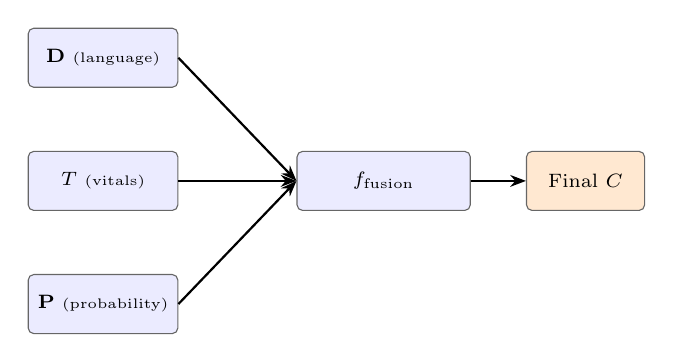
\begin{tikzpicture}[node distance=0.75cm and 0.55cm]
			\node[flowbox, minimum width=1.9cm] (d) {$\mathbf{D}$ {\tiny (language)}};
			\node[flowbox, below=0.8cm of d, minimum width=1.9cm] (t) {$T$ {\tiny (vitals)}};
			\node[flowbox, below=0.8cm of t, minimum width=1.9cm] (p) {$\mathbf{P}$ {\tiny (probability)}};
			\node[flowbox, right=1.5cm of t, minimum width=2.2cm] (ff) {$f_{\text{fusion}}$};
			\node[flowbox, right=0.7cm of ff, fill=orange!18, minimum width=1.5cm] (c) {Final $C$};
			\draw[flowarr] (d.east) -- (ff.west);
			\draw[flowarr] (t.east) -- (ff.west);
			\draw[flowarr] (p.east) -- (ff.west);
			\draw[flowarr] (ff) -- (c);
		\end{tikzpicture}}
	\end{center}

	\vspace{0.15em}
	\footnotesize Urgency order: $\mathrm{ord}(\text{Red})=4 > \mathrm{ord}(\text{Orange})=3 > \mathrm{ord}(\text{Yellow})=2 > \mathrm{ord}(\text{Green})=1$. When layers disagree, fusion picks the safer (higher) urgency.
\end{frame}

\section{Patient input}

% ========== Part III: Patient input ==========
\begin{frame}{How patients report symptoms in the chatbot}
	Users type in the \textbf{chat window} or send \textbf{voice notes}; both become symptom text $X$ for the NLP layer.

	\vspace{0.25em}
	\textbf{Typed chat:} The patient message is stored as $X$ (symptom text in English for BioBERT).

	\textbf{Voice:} Sound is converted to text, then to English:
	\[
	X = g_{\text{trans}}\!\bigl(g_{\text{ASR}}(\mathrm{audio})\bigr)
	\]
	Here $g_{\text{ASR}}$ = speech-to-text (sound $\rightarrow$ letters) and $g_{\text{trans}}$ = machine translation (e.g.\ Twi $\rightarrow$ English).

	\vspace{0.25em}
	\footnotesize One patient visit is tracked as session $s$ so all modules share the same record.
\end{frame}

\begin{frame}{Why medical English is required for BioBERT}
	BioBERT was trained on biomedical \textbf{English} (PubMed, clinical notes). The model expects input $X$ in English.

	\vspace{0.3em}
	\begin{itemize}
		\item Twi or other local languages are translated before NLP runs.
		\item Google Cloud Translation offers a free tier ($\sim$500k characters/month); \textbf{Twi may not be supported} on the API --- a glossary fallback may be needed.
	\end{itemize}

	\vspace{0.25em}
	\footnotesize Translation quality affects which danger words reach BioBERT; clinical review of common phrases is part of deployment.
\end{frame}

\section{BioBERT}

% ========== Part IV: BioBERT ==========
\begin{frame}{Turning words into vectors the model can compare}
	The tokeniser $\tau$ splits $X$ into pieces $t_1,\ldots,t_M$. Each piece gets a vector:
	\[
	E(t_i) = E_{\text{word}}(t_i) + E_{\text{pos}}(i) + E_{\text{seg}}(t_i)
	\]
	$E_{\text{word}}$ = meaning of the piece; $E_{\text{pos}}(i)$ = position in the sentence; $d=768$ is the vector size (BERT-Base). Token \texttt{[CLS]} at the start will summarise the whole message.
\end{frame}

\begin{frame}{Letting each word attend to the rest of the sentence}
	Each Transformer layer uses \textbf{self-attention} so words share context:
	\[
	\mathrm{Attention}(Q,K,V) = \mathrm{softmax}\!\left(\frac{QK^\top}{\sqrt{d_k}}\right) V
	\]
	$Q$ (query), $K$ (key), and $V$ (value) are learned projections; $d_k$ scales the scores; softmax turns them into weights summing to 1. The stack has $L=12$ layers and $H=12$ parallel heads per layer.
\end{frame}

\begin{frame}{Detecting SATS danger patterns in the text}
	The NLP function $f_{\text{NLP}}$ maps text $X$ to discriminator scores:
	\[
	\mathbf{D} = f_{\text{NLP}}(X;\,\theta_{\text{BERT}}), \qquad
	d_j = \sigma(w_j^\top h_{\texttt{[CLS]}} + b_j) \in [0,1]
	\]
	Each $d_j$ is confidence that SATS discriminator $j$ is present (e.g.\ central chest pain). If $d_j > \tau$ (e.g.\ $\tau=0.85$), that pattern counts as detected. NER = locating medical terms in $X$.
\end{frame}

\section{TEWS}

% ========== Part V: TEWS ==========
\begin{frame}{Scoring vital signs with the TEWS sum}
	\textbf{TEWS} (Triage Early Warning Score) is the deterministic function $f_{\text{TEWS}}$:
	\[
	T = f_{\text{TEWS}}(\mathbf{v}) = \sum_{k=1}^{6} w_k\, f_k(v_k), \quad w_k=1
	\]
	Vitals $\mathbf{v}$: $v_1$ mobility, $v_2$ respiratory rate (RR), $v_3$ heart rate (HR), $v_4$ temperature, $v_5$ AVPU (consciousness), $v_6$ trauma. Each $f_k(v_k)$ returns 0--3 points from SATS tables.
\end{frame}

\begin{frame}{Mapping the TEWS total to a colour band}
	Example: heart rate scoring $f_1$ when $v_1=\mathrm{HR}$:
	\small
	\[
	f_1 = \begin{cases}
		3 & \mathrm{HR} \geq 130 \\
		2 & 111 \leq \mathrm{HR} \leq 129 \\
		0 & 51 \leq \mathrm{HR} \leq 100 \\
		2 & \mathrm{HR} \leq 40
	\end{cases}
	\]

	Colour from vitals alone, $C_{\text{TEWS}}(T)$:
	\footnotesize
	\begin{tabular}{@{}ll@{}}
		$T > 7$ & \bcol[triageRed]{Red} \\
		$5 \leq T \leq 6$ & \bcol[triageOrange]{Orange} \\
		$3 \leq T \leq 4$ & \bcol[triageYellow]{Yellow} \\
		$T \leq 2$ & \bcol[triageGreen]{Green}
	\end{tabular}
\end{frame}

\section{Bayesian layer}

% ========== Part VI: Bayesian ==========
\begin{frame}{Estimating colour probability when evidence is partial}
	When vitals are missing, $f_{\text{Bayes}}$ updates beliefs:
	\[
	P(C_k \mid E) = \frac{P(E \mid C_k)\, P(C_k)}{\sum_j P(E \mid C_j)\, P(C_j)}
	\]
	$C_k$ = colour class $k$; $P(C_k)$ = \textbf{prior} (how common $k$ is at the hospital); $P(E \mid C_k)$ = \textbf{likelihood} (how often evidence $E$ appears if colour is $k$).
\end{frame}

\begin{frame}{Building evidence from symptoms and measured vitals}
	Evidence bundles language and vitals:
	\[
	E = \mathrm{concat}(\text{symptoms from NLP},\; \mathbf{v}_{\text{obs}})
	\]

	If some vitals are missing: $T_{\text{partial}} = \sum_{k \in \text{observed}} w_k f_k(v_k)$, and fusion may use $C = \arg\max_k P(C_k \mid E)$ (pick the colour with highest posterior probability).
\end{frame}

\section{Fusion rules}

% ========== Part VII: Fusion rules ==========
\begin{frame}{Applying the fusion algorithm in priority order}
	\textbf{Same rules as the Fusion section} (slide 7). $f_{\text{fusion}}$ checks in order (first match wins):
	\small
	\begin{enumerate}
		\item Red discriminator in $\mathbf{D}$ ($d_j > \tau$) $\Rightarrow$ $C =$ \bcol[triageRed]{Red}
		\item Orange discriminator in $\mathbf{D}$ $\Rightarrow$ $C =$ \bcol[triageOrange]{Orange}
		\item $T > 7$ $\Rightarrow$ $C =$ \bcol[triageRed]{Red}
		\item $5 \leq T \leq 6$ $\Rightarrow$ $C =$ \bcol[triageOrange]{Orange}
		\item $3 \leq T \leq 4$ $\Rightarrow$ $C =$ \bcol[triageYellow]{Yellow}
		\item Vitals incomplete $\Rightarrow$ $C = \arg\max_k P(C_k \mid E)$
		\item Else $C =$ \bcol[triageGreen]{Green}
	\end{enumerate}
\end{frame}

\begin{frame}{Resolving conflicts so patients are not under-triaged}
	\begin{center}
		\small
		\begin{tabular}{@{}ccc@{}}
			\toprule
			\textbf{Language} $\mathbf{D}$ & \textbf{TEWS} $T$ & \textbf{Final $C$} \\
			\midrule
			High (chest pain) & $T=4$ (Yellow alone) & \bcol[triageOrange]{Orange} \\
			Low & $T \geq 7$ & \bcol[triageRed]{Red} \\
			\bottomrule
		\end{tabular}
	\end{center}

	\vspace{0.4em}
	A strong discriminator overrides a mild $T$. High $T$ overrides weak language. Fusion always errs toward the more urgent colour when signals conflict.
\end{frame}

\section{Implementation}

% ========== Part IX: Close ==========
\begin{frame}{Data and software required to run the system}
	\small
	\begin{tabular}{@{}p{0.34\textwidth}p{0.58\textwidth}@{}}
		\toprule
		\textbf{Needed} & \textbf{Purpose} \\
		\midrule
		Patient text or audio & Input $X$ \\
		SATS tables $f_k$, $w_k$ & Compute $T$ \\
		Discriminator list & Labels for $\mathbf{D}$ \\
		Prior / likelihood tables & Bayesian $\mathbf{P}$ \\
		BioBERT weights $\theta_{\text{BERT}}$ & Run $f_{\text{NLP}}$ \\
		Session store & All layers share one record $s$ \\
		\bottomrule
	\end{tabular}
\end{frame}

\section{References}

\begin{frame}{References}
	\scriptsize
	\setlength{\itemsep}{0.15em}
	\begin{itemize}
		\item South African Triage Group (2012). \textit{The South African Triage Scale (SATS) Training Manual}. Health Professions Council of South Africa.
		\item Lee, J., Yoon, W., Kim, S., et al.\ (2020). BioBERT: a pre-trained biomedical language representation model for biomedical text mining. \textit{Bioinformatics}, 36(4), 1234--1240.
		\item Devlin, J., Chang, M.-W., Lee, K., \& Toutanova, K. (2018). BERT: Pre-training of deep bidirectional transformers for language understanding. \textit{arXiv:1810.04805}.
		\item Vaswani, A., Shazeer, N., Parmar, N., et al.\ (2017). Attention is all you need. \textit{Advances in Neural Information Processing Systems}, 30.
		\item Stewart, J., Lu, J., Goudie, A., et al.\ (2023). Applications of natural language processing at emergency department triage: A narrative review. \textit{PLOS ONE}, 18(12), e0279953.
		\item Google. \textit{Google Cloud Translation API} documentation (character quotas and language support). \url{https://cloud.google.com/translate}.
		\item Samuel, Q., \& Samuel, T. (2026). Hybrid fusion rules for the hospital triage chatbot. Final Year Project, KNUST Mathematics.
	\end{itemize}
\end{frame}

\end{document}
